\section{Modeling Online Social Networks}
\label{sec:OSN-Model}
We present a formal framework for Twins of Online Social Networks (TWONs) that captures both user behavior (Sect.~\ref{subsec:ModelingAgents}) and platform mechanics (Sect.~\ref{subsec:ModelingNetworks}). This framework enables systematic comparison between simulated and observed behaviors. Figure~\ref{fig:agent-formalization} illustrates key concepts.

\begin{figure*}
    \centering
    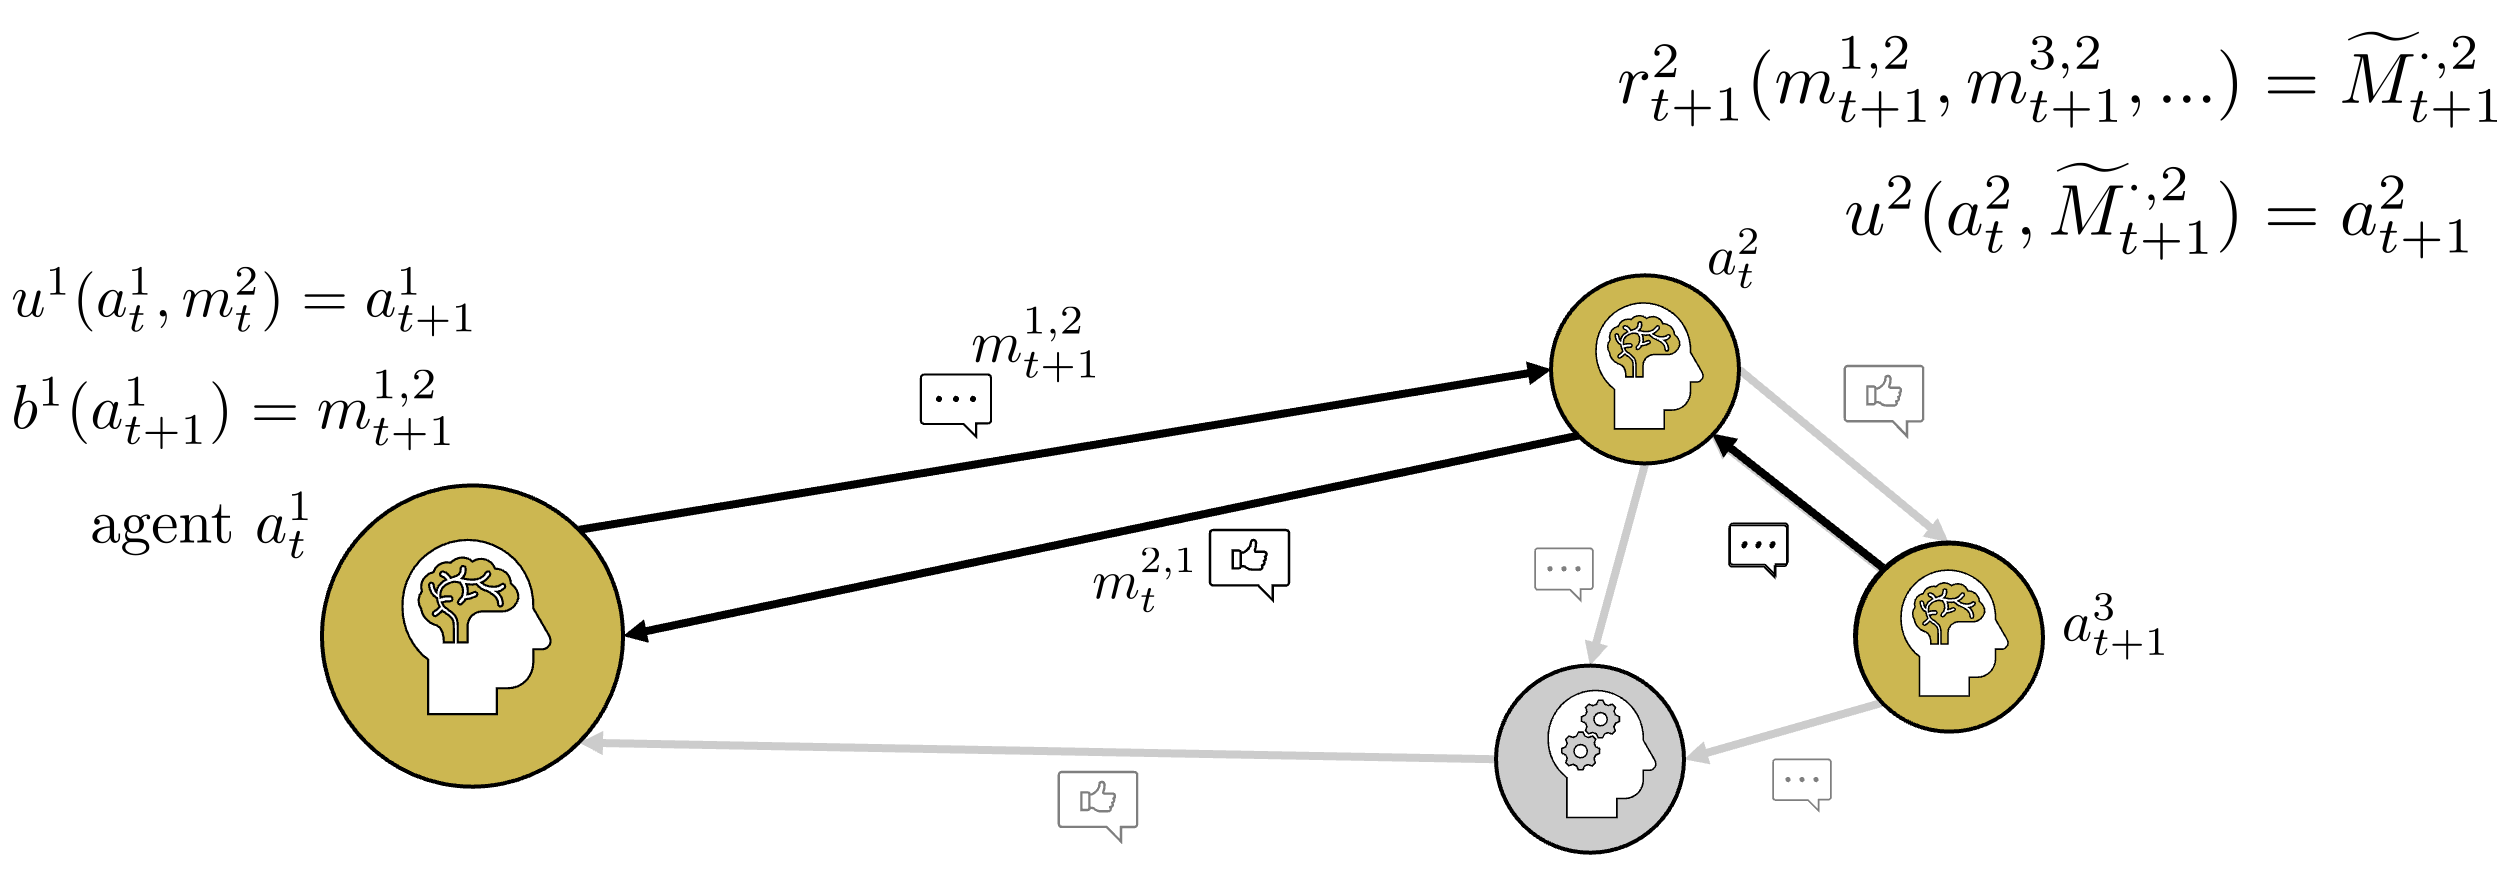
\includegraphics[width=1\linewidth]{assets/agent-formalization.png}
    \caption{
        Illustrating example:
        Agent ($a^2$) sends a message to agent ($a^1$), triggering a model update and reply generation. Agent ($a^2$) receives a curated list of incoming messages at $t+1$ and updates its model accordingly. This illustrates the interplay between agent behavior ($b$) and network mechanics ($r$).
    }
    \label{fig:agent-formalization}
\end{figure*}

\subsection{Modeling Agents}
\label{subsec:ModelingAgents}
Let $A$ be a set of agents, i.e., social media users, where $a_t^i$ is the state of the $i$-th agent at time $t$.\footnote{The internal state of an agent can be represented by symbolic logic, machine learned functions, cognitive architecture or any other agent formalism that is capable of perceiving its environment and acting upon that environment.}

$M$ is a set of messages, where $m_t^{(i,j)}$ is a message from agent $i$ to agent $j$ at time $t$. Consequently, $m_t^{(i,\cdot)}$ indicates a message that agent $i$ transmits to all other agents and $M_t^{(\cdot, i)}$ indicates all messages sent to agent $i$. Accordingly, $M_t^i$ indicates all messages that agent $i$ sends and receives at time $t$.

The state $a_t^i$ of the $i$-th agent at time $t$ is defined by the discourse it has been involved in up to this point: $(M_0^i, M_1^i,... , M_t^i)$. The agent's state is updated according to the function $u^i(a_{t}^i, M_t^i) = a_{t+1}^i$ based on its previous state and the messages sent and received since the last point in time.

The communicative behavior $b^i(\cdot)$ of the agent $i$ is a function that maps its current state $a_t^i$ to the messages $m_{t+1}^{(i,j)}$ he is sending next to agents $j$: $b^i_t(a_t^i) = M_{t}^{(i,j)}$.

\subsection{Modeling Network Mechanics}
\label{subsec:ModelingNetworks}
The mechanics of the communication channel (here, an online social network) is defined by a function $r^i_t(\cdot)$ that adapts the agent $i$' to the incoming messages $M_t^{(\cdot, i)}$ to $\widetilde{M}_t^{(\cdot, i)}$, returning a manipulated list of messages. Standard manipulations of the list are filtering or ranking, but could also include the manipulation of content or the addition of messages to the list that have not been directly sent between agents. Note that this function can be personalized and be adapted over time.
%\footnote{Personalized content curation based on machine-learned recommender systems is standard in social nets.}.

In general, the messages agent $i$ receives at time $t$ are given by:
% $$ \widetilde{M}_{t+1}^{(\cdot, i)} = r^i( b^{j}_t(a^j) ) \mbox{ for all agents } j \mbox{ sending } m_{t+1}^{(j, i)}  $$

% $$ \widetilde{M}_{t+1}^{(\cdot, i)} = r_t^i( b^{j}_t(a_t^j) ) \quad \forall j \in m_{t+1}^{(j, i)} \quad i \neq j  $$

% $$ \widetilde{M}_{t+1}^{(\cdot, i)} = r^i( b^{j}_t(a^j) ) \quad \forall M_{t+1}^{(j, i)}  $$

$$ r_t^i( b^{j}_t(a_t^j)) = \widetilde{M}_{t}^{(\cdot, i)} \quad \forall j \in A_t^j  $$

% $$ \widetilde{M}_{t+1}^{(\cdot, i)} = r_t^i( b^{j}_t(\widetilde{M}_{t}^{(\cdot, j)}) ) \ \forall j \in A_t^j  $$


which in turn triggers agent $i$s response 

$$ b^i_{t+1}( u^i(a^i_t, \widetilde{M}_{t}^{(\cdot, i)})) = M_{t+1}^{(i,\cdot)}$$

\section{Simulating TWONs}
\label{sec:replication}
Based on the formal framework introduced in Sect.~\ref{sec:OSN-Model} we define the required tasks to construct a TWON by replicating its behavior at the user (Sect.~\ref{subsec:replicatingUsers}) and system level (Sect.~\ref{subsec:replicatingUsers}). Finally, this allows us to check the empirical realism of such TWONs (Sect.~\ref{subsec:simulation}).

\begin{table*}[ht]
	\centering
    \small
	\begin{tabular}{l | llllll}
		\toprule
		Behavior $b$ & 
        Agent $a^i$  & 
        Task Type & 
        Input $\widetilde{M}_{t}^{(\cdot, i)}$ & 
        Output $m_{t+1}^{(i,\cdot)}$ & 
        Loss $L_b$ &
        Metric(s) $q$ \\
		\midrule
		Posting & Creator & Generative  & Topic  & Free Text & Cross Entropy & BLEU, ngram,... \\
		Replying & Reactor & Generative  & Post   & Free Text & Cross Entropy & BLEU, ngram,... \\
		Replying Likelihood & Reactor & Probability & Post & Interval [0,1] & Binary Cross Entropy & F1, Acc. \\
%		(Dis-)Liking Likelihood & Reactor & Similarity  & Post & Interval [-1,1] & \textit{untrained} & Cosine Similarity \\
		\bottomrule
	\end{tabular}
    \vspace{0.1cm}
	\\
%	\footnotesize{
 %       All get tasks have the user history as main stimulus and in addition the defined input
%    }
	\caption{Communicative behaviors modeled, imitated and benchmarked in our empirical study with respect to their empirical realism, as definied in our formal framework.}
	\label{tab:methods:task}
\end{table*}

\paragraph{Imitating User Behavior}
\label{subsec:replicatingUsers}
The task of machine learning an agent-based simulation of human social media communication behavior at user level is to estimate the function $b^i(\cdot)$ of each agent $i$, which given real-world observations of discourses $(M_0^i, M_1^i,... , M_t^i)$ predicts its next message $m_{t+1}^i$. Thus, the objective can be formulated as minimizing a loss function 

$$\textrm{min\ } L_{b}(\widehat{m}_{t+1}^i, m_{t+1}^i) \mapsto \mathbb{R}$$

that compares the predicted $\widehat{m}_{t+1}^i$ to its observed value.\footnote{Any text comparison metric, like BLEU, cross-entropy, but also higher level metrics could be applied here. In addition, other metrics can be used to measure the predictive accuracy of discrete actions such as "liking".}

\paragraph{Replicating Network Mechanics}
\label{subsec:replicatingMechanics}
The task of replicating the system-level mechanics of a social network from observations is to estimate the function $r^i$ of each agent $i$, given its observed messages $(\widetilde{M}_1^i, \widetilde{M}_1^i,... , \widetilde{M}_t^i)$.

This objective can be formulated as minimizing the loss 

$$\textrm{min\ } L_{r}(\widehat{M}_t^{(\cdot, i)}, \widetilde{M}_t^{(\cdot, i)}) \mapsto \mathbb{R}$$

that compares the predicted $\widehat{M}_t^{(\cdot, i)}$ with its observed value.

\paragraph{Simulating Social Networks}
\label{subsec:simulation}
Finally, a simulation task for investigating user communication on social networks can be stated as follows: Given (an estimation of) $b$ and $r$ generate a discourse $M_{t+1}, ..., M_{t+n}$ and evaluate it according to a discourse metric $q$, for example, the degree of outrage or hate speech, mapping 
$$q(M_{t+1}, ..., M_{t+n}) \mapsto \mathbb{R}$$

Any findings obtained by $q$ can be put into perspective by $L_{b}$ and $L_{r}$ as they quantify the empirical realism of the simulation of a social network and consequently qualify the validity of $q$. $L_{b}$ and $L_{r}$ can be interpreted as a confidence score for any empirical findings obtained by simulating social networks and should be reported together with empirical findings obtained by simulation.

